\acrfull{cdh} and telecommunications form an integral part of the avionics system. These perform four functions: flight and vehicle control, data processing, human interfacing and communications \cite{Eger2008}. This requires a direct link to the \gls{adcs} module, a link to the telecommunications network and a link to on-board display for crew members. These are illustrated in Figure \ref{fig:cdhflow}

\begin{figure}[h]
		\centering
		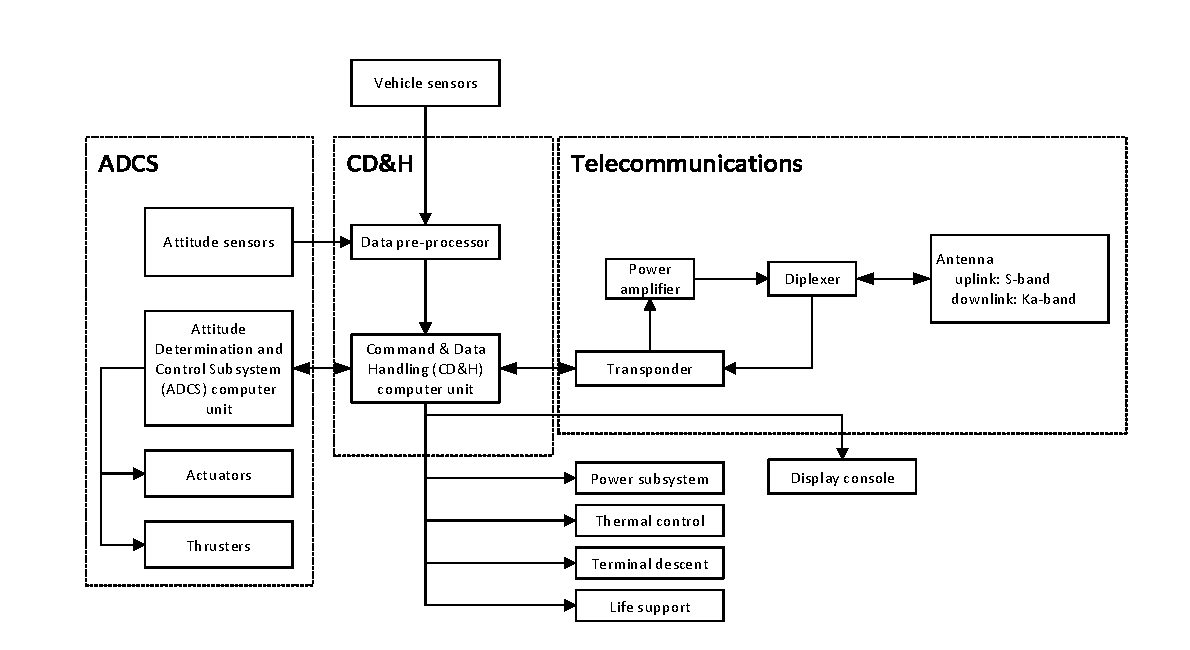
\includegraphics[width=0.95\textwidth]{./Figure/CrewModule/CDH.pdf}
		\vspace{-12mm}
		\caption{Communication flow}
		\label{fig:cdhflow}
\end{figure}

Data processing is performed as follows. Data is first filtered, then analysed to see if reactions are required and in case reactions are required put through to the relevant effectors (subsystems) and critical system information communicated to the ground station via the Ka-band (see section \ref{sec:groundop}). Modulation is performed in the transponder by \gls{bpsk} on the carrier and subcarrier (modulating the carrier) and \gls{qpsk} on the carrier, similar to the Mars Reconnaissance Orbiter mission \cite{Taylor2006}.

For its integral part, it is key that the system is redundantly equipped to ensure adequate system reliability. To this end, cabling is redundant and safety-critical processing tasks are performed by self-checking pair processors, following their application in Orion \cite{Eger2008}. These self-checking pair processors observe and compare the activity of their partner to identify faulty behaviour. 

Antennas used can be extracted from a reference mission to Mars, for example the Mars Reconnaissance Orbiter \cite{Taylor2006}. This mission had relatively high scientific return communications and used a $3$ [$m$] diameter high gain antenna and two low gain antennas. The communication system for this mission was remarkable because it was able to send data back to Earth more than ten times faster than previously conducted missions. Such a high return would be highly beneficial for the manned mission at hand to maximize ground surveillance possibilities and accurate monitoring. It similarly used Ka-band communication for downlink. To this end, the communication system is deemed a good reference system for use in the mission at hand.

The mass of the \gls{cdh} subsystem is extrapolated from that in the Mars Odyssey mission by scaling with the ratio of masses. For a $11.1$ [$kg$] \gls{cdh} subsystem mass in the 376 [$kg$] Mars Odyssey\footnote{URL:\url{http://mars.nasa.gov/odyssey/mission/spacecraft/parts/command/}. Accessed: 11-06-2015}, this translates to nearly $300$ [$kg$] on the $10,000$ [$kg$] entry vehicle at hand. This telecommunications system had a mass of $108$ [$kg$], which is not scaled since the sizing thereof is not deemed mass-dependent. Taking into account a contingency for the larger crew module and more demanding mission at hand as well as the roughness of the estimates, the \gls{cdh} and telecommunications mass is estimated at $530$ [$kg$], thus taking a $30$ $\%$ contingency into account. In addition, cabling requires additional contingency, taken to be $10$ $\%$ and a mass of $53$ [$kg$].
